\documentclass[12pt]{article}
\usepackage[utf8]{inputenc}
\usepackage[T1]{fontenc}
\usepackage{fontspec}
\setmainfont{Times New Roman}
\newfontfamily\hackfont{Hack}
\usepackage{titlesec}
\usepackage{fancyhdr}
\usepackage{listings}
\usepackage{xcolor}
\usepackage{graphicx}
\usepackage{longtable}
\usepackage{caption}
\usepackage{hyperref}
\usepackage{setspace}
\usepackage{geometry}
\geometry{a4paper, margin=1in}
\renewcommand{\contentsname}{Table of Contents}
\hypersetup{colorlinks=true, linkcolor=black, urlcolor=blue}


\pagestyle{fancy}
\fancyhf{} 							% Header Middle
\rhead{Computer Networks Lab}
\lhead{Hardware Lab Report}
\rfoot{\thepage}

\begin{document}

\begin{titlepage}					% Cover Start
\begin{center}
    
\includegraphics[width=0.35\textwidth]{logo.png} \\
    \vspace{0.5cm}
    \textbf{\Huge \textcolor{teal}{NOTRE DAME} \textcolor{teal}{UNIVERSITY}} \\
    \vspace{0.5cm}
    \textbf{\Huge \textcolor{orange}{BANGLADESH}} \\
    
    \vspace{0.9cm}
    \textbf{\Huge \underline{Computer Networks Hardware Lab Report}} \\
    
    \vspace{1.5em}
    \begin{flushleft}
    	\textbf{\Large Course Code: CSE-3204} \\
		\vspace{0.3cm}        
        \textbf{\Large Course Title: Computer Networks Lab} \\
        \vspace{0.3cm}
        \textbf{\Large Lab Task Topic: Introduction to Hardware Equipments} \\        
    \end{flushleft}
    
    \vspace{1em}
    \begin{flushleft}
        \textbf{\Huge \textcolor{blue}{Submitted by:}} \\
        \vspace{0.3cm}
        \textbf{\Large Name: Istiak Alam} \\
        \vspace{0.3cm}
        \textbf{\Large ID: 0692230005101005} \\
		\vspace{0.3cm}        
        \textbf{\Large Batch: CSE-20} \\
        \vspace{0.5cm}
        \textbf{\Large Submission Date: }{\Large \textbf{\today}\par}
    \end{flushleft}
    \vfill
    \begin{flushleft}
        \textbf{\Huge \textcolor{blue}{Submitted to:}} \\
        \vspace{0.3cm}
        \textbf{\Large Dr. Fernaz Narin Nur} \\
        \vspace{0.3cm}
        \textbf{\Large Adjunct Professor,} \\
        \vspace{0.3cm}
        \textbf{\Large Notre Dame University Bangladesh}
    \end{flushleft}
\end{center}
\end{titlepage}						% Cover End

\tableofcontents
\thispagestyle{empty}
\clearpage
\pagenumbering{arabic}

\begin{abstract}
This lab report provides a comprehensive overview of essential computer networking hardware components and configurations encountered in practical networking environments. The main objective of this lab was to familiarize students with various networking tools and equipment such as cable testers, cable tracers, RS-232 cables, fiber optic duplex cables, SFP modules, and to understand the physical and logical aspects of network devices like switches and routers.\\
Through hands-on activities, we learned how to identify, test, and properly connect network cables using T-568B wiring standards, configure routers for Dynamic NAT and DHCP, and establish effective connections between switches and routers. The report also discusses the conceptual framework of the OSI Model to better understand the layer-wise interaction of network protocols and hardware.\\
By engaging in these exercises, students developed a strong foundational understanding of how computer networks are physically built and logically managed, which is crucial for further studies and careers in networking and IT infrastructure. The inclusion of real-world scenarios and step-by-step procedures reinforced the theoretical knowledge with practical implementation, bridging the gap between textbook learning and field expertise.\\
\end{abstract}


\section*{Introduction}
\addcontentsline{toc}{section}{Introduction}
The rapid growth of computer networks and internet-based technologies has significantly increased the demand for reliable and high-performance network infrastructure. Understanding the physical hardware components that form the foundation of such networks is essential for any networking professional or student. This lab report provides a comprehensive overview of various fundamental hardware tools and equipment used in networking environments.

In this report, we explore the practical application and functionality of essential devices such as cable tracers, cable testers, RS-232 cables, fiber optic duplex cables, and SFP modules. We also study network components like switches and routers, along with their configurations and interconnections. A key focus is placed on the T-568B Ethernet cabling standard, which defines the proper arrangement of wire pairs in twisted-pair cables for effective network communication.

Additionally, the report covers the Open Systems Interconnection (OSI) model, a conceptual framework that categorizes and standardizes the functions of a communication system into seven distinct layers. Each hardware topic is supported with descriptions and relevant images to aid in practical understanding.

This lab aims to enhance student's hands-on skills in identifying, using, and configuring networking hardware, thereby building a strong foundation for designing and managing robust network systems.

\newpage

\section{Cable Tracer}
A \textbf{Cable Tracer} is an essential diagnostic tool used in computer networking to detect and follow the physical route of cables, especially in complex or hidden wiring environments. It is most commonly used during network installation, troubleshooting, and maintenance to identify the exact path and endpoints of cables such as twisted pair (Ethernet), coaxial, or telephone wires.
The cable tracer typically consists of two main components: 
\begin{itemize}
    \item \textbf{Tone Generator (Transmitter)} – This device sends a low-voltage signal through the cable under test.
    \item \textbf{Probe (Receiver)} – This hand-held device detects the electromagnetic signal emitted from the cable, allowing technicians to follow its path.
\end{itemize}

\begin{center}
    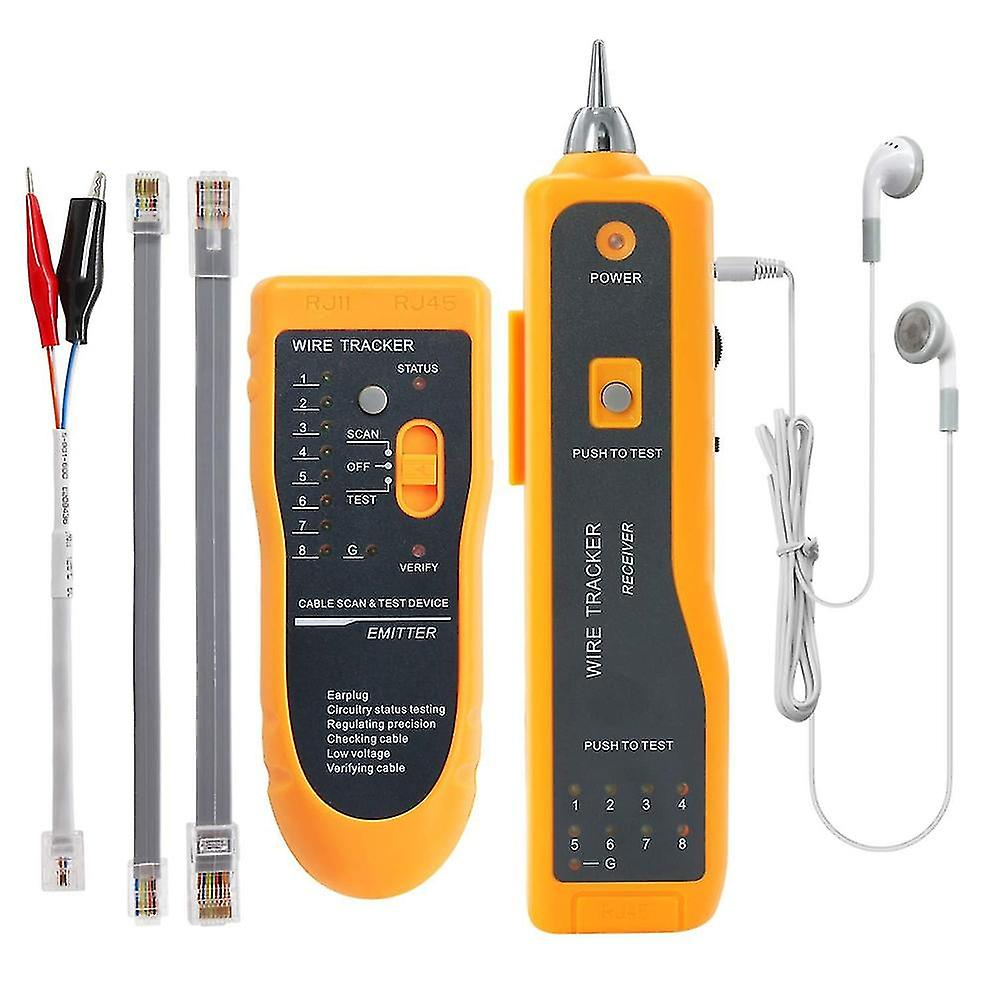
\includegraphics[width=0.3\textwidth]{CableTracer.jpg} \\
    {\small \textbf{Figure 1:} Cable Tracer}
\end{center}

\subsection{Working Principle}  
The tone generator is connected to one end of the cable, and it emits a specific frequency. The technician then moves the receiver probe along the suspected cable route. The probe produces an audible tone that gets louder as it nears the cable carrying the signal, helping to trace the cable's direction through walls, ceilings, or cable trays.

\subsection{Usage in Lab}  
In our lab exercise, the cable tracer was used to identify and trace Ethernet cables running between workstations and the central switch panel. This was particularly useful in verifying that each workstation was correctly connected to the intended switch port. We also practiced identifying disconnected or mislabeled cables using the tone and probe method. This exercise demonstrated the importance of cable management and verification in real-world networking environments.

\subsection{Advantages}
\begin{itemize}
    \item Helps in quickly identifying cable paths without disconnecting network devices.
    \item Useful in locating broken or damaged cables within walls or conduits.
    \item Saves time during troubleshooting and network deployment.
\end{itemize}


\section{Cable Tester}
A \textbf{cable tester} is an essential diagnostic tool used in computer networking to test the physical integrity and wiring configuration of network cables, particularly twisted-pair Ethernet cables terminated with RJ-45 connectors. The main purpose of a cable tester is to identify issues such as open circuits, short circuits, crossed wires, miswiring, and split pairs that can disrupt data transmission.
Cable testers typically consist of two units:
\begin{itemize}
    \item \textbf{Main Unit (Transmitter)}: Sends electrical signals through each wire in the cable.
    \item \textbf{Remote Unit (Receiver)}: Receives the signal and verifies whether each wire is correctly terminated.
\end{itemize}

\begin{center}
    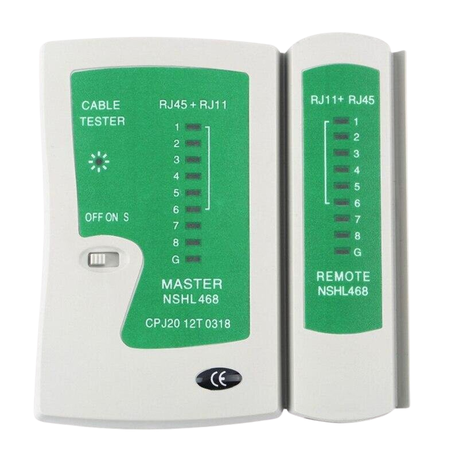
\includegraphics[width=0.3\textwidth]{CableTester.jpg} \\
    {\small \textbf{Figure 2:} Cable Tester}
\end{center}
The cable tester visually displays the status of each pin via a row of LED indicators. If the cable is wired correctly (e.g., using the T-568B standard), all LEDs light up in a sequential and matching order on both ends. If there is a wiring error, such as a missing connection or reversed pair, the LEDs will either not light up or show an incorrect sequence.

\subsection{Usage in Lab}  
During our networking hardware lab session, we used the cable tester to verify the integrity of custom-made Ethernet cables. After crimping RJ-45 connectors onto CAT5e cables following the T-568B wiring standard, we connected each end of the cable to the main and remote units of the tester. The LED lights helped us confirm whether all eight wires were correctly connected. If the lights did not match the correct pattern, we identified the faulty end and re-crimped the connector.

\subsection{Benefits}
\begin{itemize}
    \item Saves time during troubleshooting by quickly identifying bad cables.
    \item Ensures that cables meet required standards before connecting them to network devices.
    \item Reduces network downtime caused by faulty or miswired cables.
\end{itemize}
Overall, the cable tester is a valuable tool in both academic and professional networking environments for ensuring reliable physical layer connectivity.


\section{T-568B Wiring Standard}

The \textbf{T-568B Wiring Standard} is one of the two recognized wiring configurations for terminating Ethernet cables using RJ-45 connectors. It defines the pin-out order the sequence of wire colors for the eight conductors inside a twisted-pair Ethernet cable. The standard is defined by the Telecommunications Industry Association (TIA) and is used to ensure uniformity and compatibility across network devices and installations. \textbf{Color Order : wo-o-wg-b-wb-g-wc-c}

\subsection{Color Code Order}
The color sequence for the T-568B standard, from pin 1 to pin 8, is as follows: 
\begin{center}
    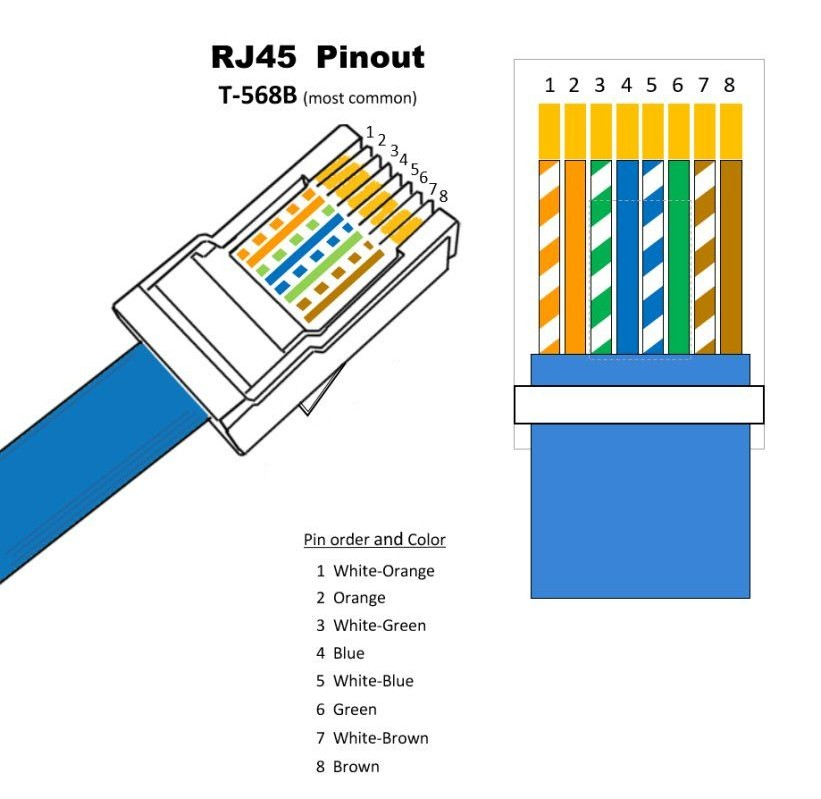
\includegraphics[width=0.4\textwidth]{WireStandard.jpg} \\
    {\small \textbf{Figure 3:} Wiring Standard}
\end{center}
Each pair of colors represents a twisted pair of wires. The T-568B configuration places specific twisted pairs on specific pins to reduce cross-talk and ensure proper signal transmission.

\subsection{Applications}
The T-568B wiring standard is widely used in both residential and commercial Ethernet installations. It is compatible with modern networking equipment like switches, routers, and network interface cards (NICs). While both T-568A and T-568B are acceptable under ANSI/TIA standards, T-568B is more popular in the United States, especially in data installations.

\subsection{Straight-Through and Crossover Cables}
\textbf{Straight-through Cable:} Both ends of the cable use the T-568B wiring configuration. Used to connect dissimilar devices, such as a PC to a switch or a router to a modem. \\
\textbf{Crossover Cable:} One end uses T-568A and the other T-568B. Used to connect similar devices, such as switch-to-switch or PC-to-PC connections.


\subsection{Importance in Lab}
In our lab activities, we used the T-568B standard while crimping RJ-45 connectors onto Ethernet cables. This ensured consistency and correct connectivity throughout our network setup. The cables were then tested using a cable tester to confirm that all wires were correctly placed according to the T-568B configuration.

\section{RS-232 Cable}

The \textbf{RS-232 cable}, also known as a \textbf{serial cable}, is a standard communication cable used for \textbf{serial communication} between computers and peripheral devices. It is based on the \textbf{Recommended Standard 232 (RS-232)} developed by the \textbf{Electronic Industries Association (EIA)}, which defines the electrical characteristics and timing of signals, as well as the size and pin-out of connectors.

\subsection{Purpose and Function}
RS-232 cables are used to transmit \textbf{data serially (bit-by-bit)} between devices, typically between \textbf{Data Terminal Equipment (DTE)} like computers and \textbf{Data Communication Equipment (DCE)} like modems, printers, or routers. It is most commonly used for:
\begin{itemize}
  \item Configuration of routers and switches via \textbf{console ports}
  \item Connection to serial modems
  \item Communication between PCs and embedded systems
  \item Debugging and monitoring microcontrollers
\end{itemize}

\subsection{Physical Characteristics}
\begin{itemize}
  \item \textbf{Connectors}: RS-232 typically uses \textbf{DB9 (9-pin)} or \textbf{DB25 (25-pin)} connectors.
  \item \textbf{Cable type}: Unshielded twisted pair (UTP) or shielded cables depending on environment.
  \item \textbf{Voltage levels}: Logic levels are represented by \textbf{\textpm3V to \textpm15V} (where +3 to +15V = logic 0 and -3 to -15V = logic 1).
\end{itemize}

\subsection{Pin Configuration (DB9)}
\begin{table}[h!]
\centering
\begin{tabular}{|c|l|l|}
\hline
\textbf{Pin} & \textbf{Signal Name} & \textbf{Description} \\
\hline
1 & DCD (Data Carrier Detect) & Detects modem connection \\
2 & RXD (Receive Data) & Data received by DTE \\
3 & TXD (Transmit Data) & Data sent by DTE \\
4 & DTR (Data Terminal Ready) & DTE is ready to communicate \\
5 & GND (Ground) & Common reference ground \\
6 & DSR (Data Set Ready) & DCE is ready to communicate \\
7 & RTS (Request to Send) & DTE requests transmission \\
8 & CTS (Clear to Send) & DCE is ready to receive \\
9 & RI (Ring Indicator) & Telephone ring indicator \\
\hline
\end{tabular}
\caption{RS-232 DB9 Pin Configuration}
\end{table}

\begin{center}
    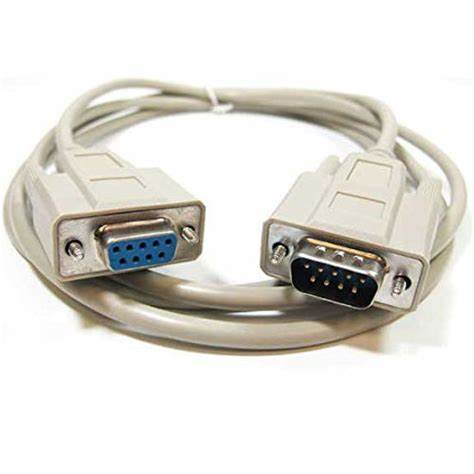
\includegraphics[width=0.4\textwidth]{OIP.jpeg} \\
    {\small \textbf{Figure 4:} RS-232 Cable}
\end{center}

\subsection{Communication Standard}
\begin{itemize}
  \item \textbf{Baud Rate}: Typically from \textbf{9600 to 115200 bps}.
  \item \textbf{Synchronous vs Asynchronous}: RS-232 uses \textbf{asynchronous communication}, where start and stop bits define each byte.
  \item \textbf{Distance Limitation}: Reliable communication is possible up to \textbf{15 meters (50 feet)}.
\end{itemize}

\subsection{Use in Lab}
In networking hardware labs, RS-232 cables are often used to:
\begin{itemize}
  \item Connect PCs to routers or switches through the \textbf{console port}.
  \item Access command-line interfaces (CLI) using terminal software like \textbf{PuTTY}, \textbf{Tera Term}, or \textbf{Cisco Packet Tracer Terminal}.
  \item Perform initial configuration, IP assignment, and troubleshoot when no network access is available.
\end{itemize}

\newpage

\section{Fiber Optic (Duplex) Cable}

Fiber optic cables are a critical component of modern high-speed communication networks. They use light signals to transmit data over long distances with minimal loss and electromagnetic interference. A \textbf{duplex fiber optic cable} consists of two optical fibers: one for transmitting (Tx) and one for receiving (Rx) data. This allows for simultaneous two-way communication, making duplex cables ideal for full-duplex networking.

\subsection{Structure and Composition}
Each fiber in the duplex cable is typically composed of:
\begin{itemize}
    \item \textbf{Core:} The innermost glass or plastic region where light is transmitted.
    \item \textbf{Cladding:} Surrounds the core and reflects light back into the core using a lower refractive index.
    \item \textbf{Buffer Coating:} Protects the fiber from moisture and physical damage.
    \item \textbf{Outer Jacket:} Provides additional protection and structural integrity.
\end{itemize}

Duplex cables are often color-coded or labeled for easier installation and maintenance, with connectors on both ends, such as LC, SC, or ST types.

\begin{center}
    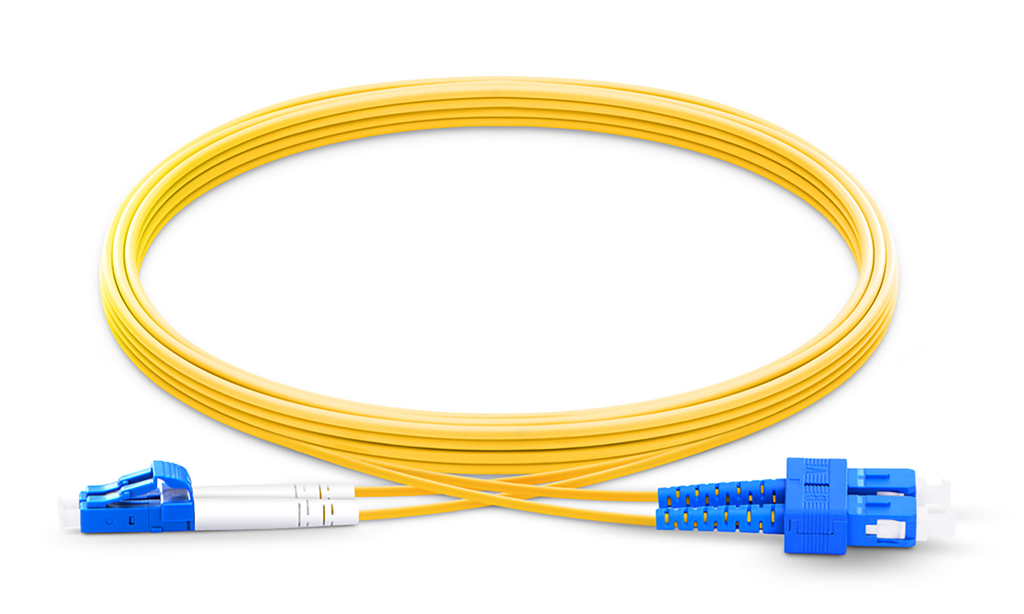
\includegraphics[width=0.4\textwidth]{FOP.png} \\
    {\small \textbf{Figure 5:} Fiber Optic Cable}
\end{center}

\subsection{Types of Fiber}
There are two main types of fiber used in duplex cables:
\begin{itemize}
    \item \textbf{Single-mode Fiber (SMF):} Used for long-distance communication, has a small core and transmits infrared laser light (wavelength ~1310 or 1550 nm).
    \item \textbf{Multi-mode Fiber (MMF):} Used for short-distance communication, has a larger core and transmits LED light (wavelength ~850 or 1300 nm).
\end{itemize}

\subsection{Applications in Networking}
\begin{itemize}
    \item Backbone connections in LANs and WANs
    \item Internet Service Provider (ISP) infrastructures
    \item Data centers and server farms
    \item High-speed long-distance communication
\end{itemize}

\section{SFP Module}

The \textbf{Small Form-factor Pluggable (SFP)} module is a compact, hot-swappable transceiver used in network hardware for both telecommunication and data communication applications. It is designed to provide flexibility in network configuration and scalability by supporting various communication standards, such as Ethernet, Fibre Channel, and SONET/SDH.

\subsection{Functionality}
An SFP module acts as an interface between a network device (like a switch or router) and a fiber optic or copper network cable. It enables the device to send and receive data over different types of media by converting electrical signals to optical signals (or vice versa) depending on the media type.

\begin{center}
    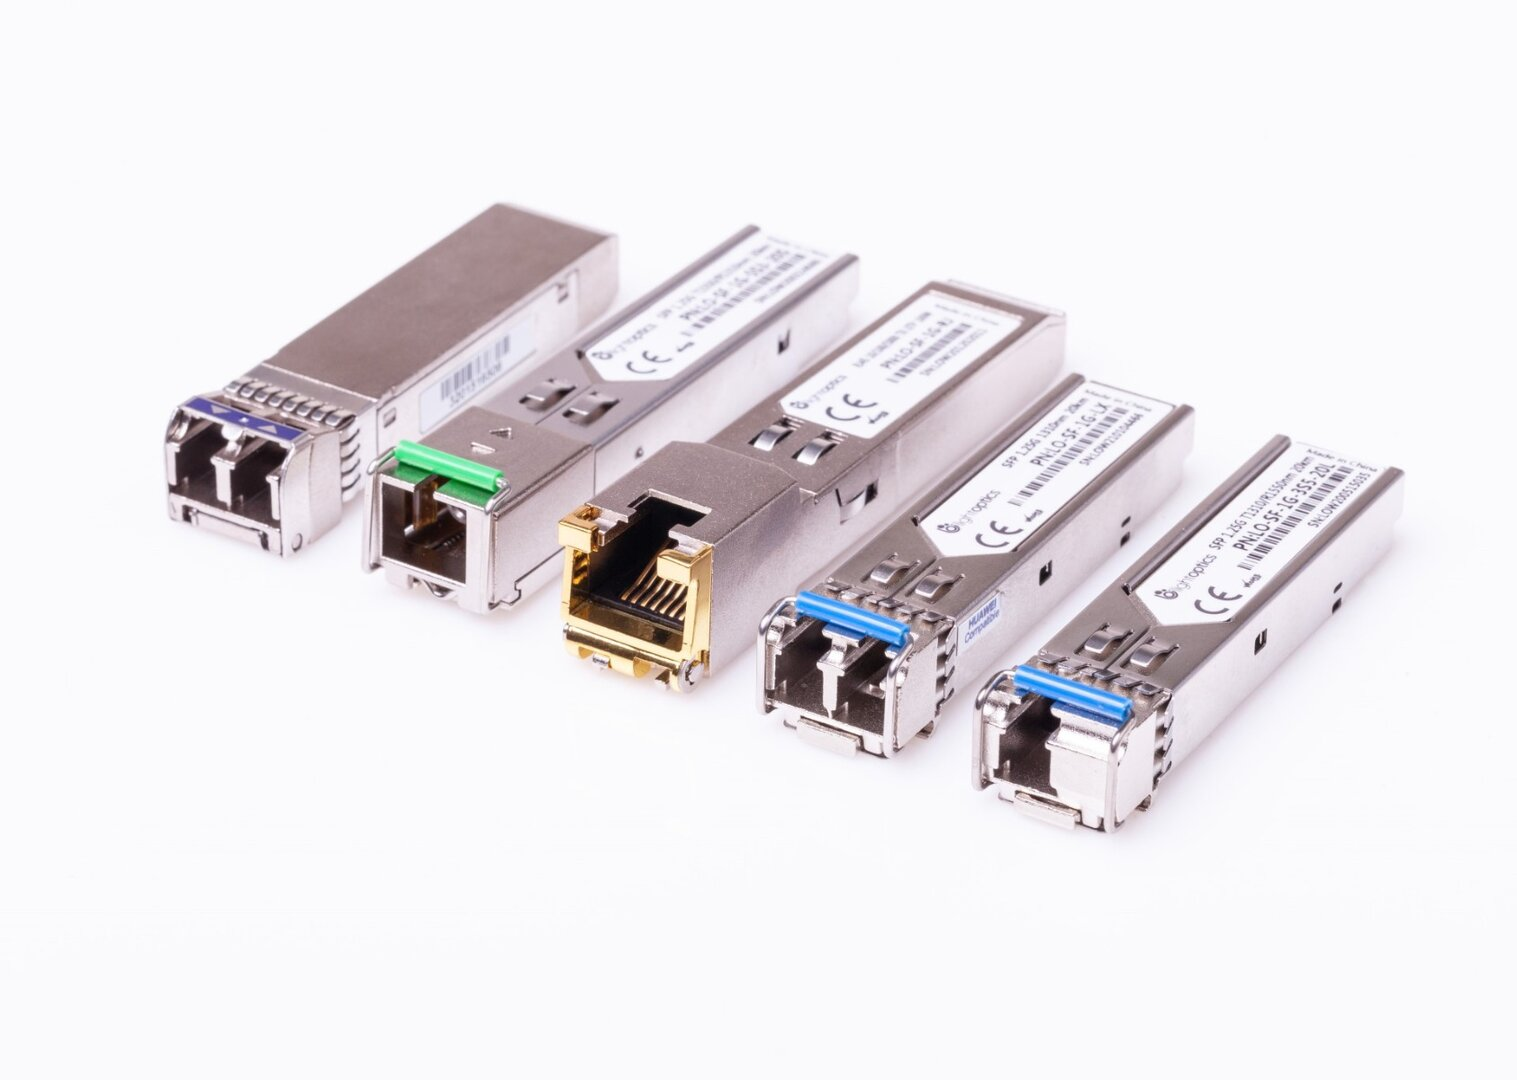
\includegraphics[width=0.4\textwidth]{sfp.jpg} \\
    {\small \textbf{Figure 6:} SFP Module}
\end{center}

\subsection{Types of SFP Modules}
There are several types of SFP modules available, depending on speed, range, and transmission medium:
\begin{itemize}
    \item \textbf{SX (Short Wavelength)} – Typically used for short-range communication over multi-mode fiber.
    \item \textbf{LX (Long Wavelength)} – Designed for long-range communication over single-mode fiber.
    \item \textbf{ZX (Extended Range)} – Supports even longer distances using single-mode fiber.
    \item \textbf{Copper SFP (RJ-45)} – Used for Gigabit Ethernet over twisted pair copper cabling.
\end{itemize}


\subsection{Applications in Networking}
SFP modules are widely used in:
\begin{itemize}
    \item Data centers
    \item Enterprise backbone links
    \item Telecommunication networks
    \item Campus LANs and WANs
\end{itemize}

\section{Switch}
A \textbf{network switch} is a fundamental device in computer networking that connects multiple devices (such as computers, printers, and servers) within a Local Area Network (LAN) and facilitates efficient data communication between them. It operates at the \textbf{Data Link Layer (Layer 2)} of the OSI model but can also support Layer 3 routing functions in advanced models.

\subsection{Functionality}
Unlike a hub, which broadcasts data to all ports, a switch is intelligent—it learns the MAC addresses of connected devices and forwards data only to the appropriate port based on the destination MAC address. This improves network efficiency and reduces unnecessary data traffic.

\subsection{Types of Switches}
\begin{itemize}
    \item \textbf{Unmanaged Switch:} Plug-and-play device with no configuration needed; commonly used in home or small office networks.
    \item \textbf{Managed Switch:} Provides advanced features like VLANs, SNMP monitoring, port mirroring, and security settings; ideal for enterprise-level networks.
    \item \textbf{Layer 3 Switch:} Combines the functions of a router and switch, capable of performing routing functions based on IP addresses.
\end{itemize}

\begin{center}
    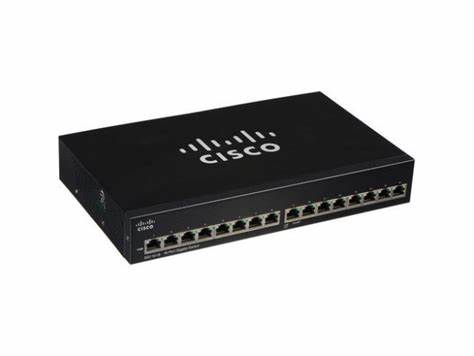
\includegraphics[width=0.4\textwidth]{switch.jpeg} \\
    {\small \textbf{Figure 7:} Switch}
\end{center}

\subsection{Applications in Networking}
\begin{itemize}
    \item Core component of LAN infrastructure
    \item Used in data centers to connect servers and storage
    \item Supports security and traffic management in enterprise networks
\end{itemize}

\subsection{Importance in Lab}
In our laboratory, network switches were used to interconnect multiple PCs and routers to form a structured LAN. We configured VLANs on managed switches to simulate departmental segmentation and observed how switches learn MAC addresses to forward frames efficiently. This provided hands-on experience in designing scalable and structured networks.


\section{Router Configuration}
A \textbf{router} is a networking device that connects different networks together and directs data packets between them. It operates primarily at the \textbf{Network Layer (Layer 3)} of the OSI model and is responsible for routing packets based on IP addresses. Router configuration is a critical task in network design, allowing proper communication, traffic control, and access between different segments of a network.

\subsection{Basic Router Configuration Tasks}
Router configuration typically involves several essential tasks, which can be performed via the router's Command Line Interface (CLI). The most common configuration steps are:

\begin{enumerate}
    \item \textbf{Accessing the CLI:} Connect to the router using a console cable and open a terminal emulator or use console access in network simulators like Cisco Packet Tracer.
    \item \textbf{Entering Privileged Mode:}
    \begin{verbatim}
    Router> enable
    \end{verbatim}
    
    \item \textbf{Entering Global Configuration Mode:}
    \begin{verbatim}
    Router# configure terminal
    \end{verbatim}
    
    \item \textbf{Setting the Hostname:}
    \begin{verbatim}
    Router(config)# hostname R1
    \end{verbatim}
    
    \item \textbf{Configuring Interfaces:}
    Assign IP addresses to interfaces and enable them.
    \begin{verbatim}
    R1(config)# interface gig0/0
    R1(config-if)# ip address 192.168.1.1 255.255.255.0
    R1(config-if)# no shutdown
    \end{verbatim}
    
    \item \textbf{Setting a Default Route (Optional):}
    Used when the router needs to forward unknown destination packets.
    \begin{verbatim}
    R1(config)# ip route 0.0.0.0 0.0.0.0 192.168.1.254
    \end{verbatim}
    
    \item \textbf{Saving Configuration:}
    \begin{verbatim}
    R1# write memory
    \end{verbatim}
\end{enumerate}

\begin{center}
    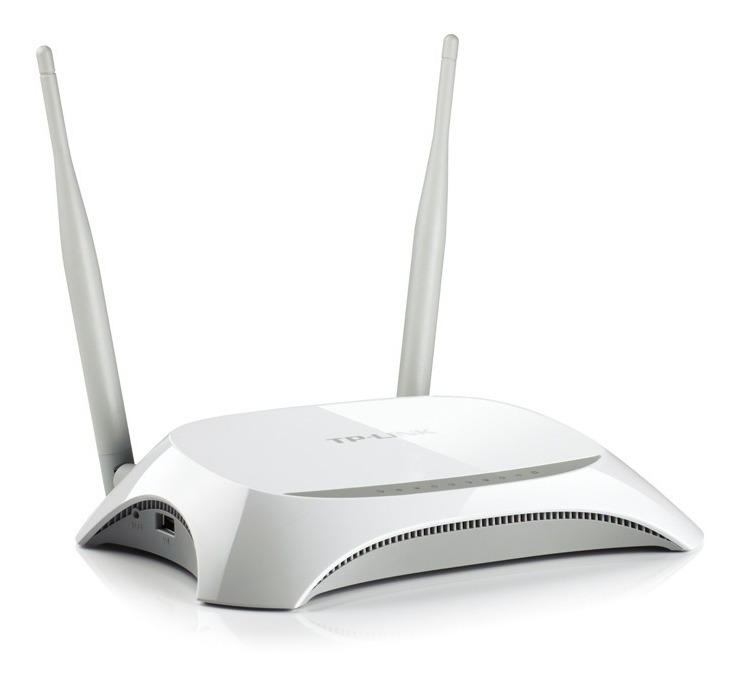
\includegraphics[width=0.4\textwidth]{router.jpeg} \\
    {\small \textbf{Figure 8:} Router}
\end{center}

\subsection{Advanced Configuration Examples}
\begin{itemize}
    \item \textbf{Dynamic Routing Protocols (like RIP):}
    \begin{verbatim}
    R1(config)# router rip
    R1(config-router)# version 2
    R1(config-router)# network 192.168.1.0
    \end{verbatim}
    
    \item \textbf{NAT Configuration:}
    Configure NAT to translate private IP addresses to public ones.
    \item \textbf{DHCP Configuration:}
    Routers can be configured to act as DHCP servers in small networks.
\end{itemize}

\subsection{Importance in Lab}
In our Computer Network Hardware Lab, routers were configured to simulate real-world network scenarios. Tasks included setting up IP addresses on interfaces, configuring static and dynamic routing, enabling NAT, and establishing inter-VLAN routing. Through these configurations, we gained practical experience in how routers manage traffic between networks and ensure communication across different subnets.

\newpage

\section{Switch to Router Connection}

In computer networking, connecting a switch to a router is a fundamental setup for enabling communication between local area network (LAN) devices and external networks (such as the internet). This configuration is also known as a \textbf{Router-on-a-Stick} setup when involving VLANs. The switch and router work together to forward traffic, manage network segmentation, and provide routing capabilities.

\subsection{Purpose of Switch to Router Connection}
\begin{itemize}
    \item To allow hosts connected to the switch to communicate with devices in other networks.
    \item To route traffic between different VLANs when VLANs are configured on the switch.
    \item To provide internet access to LAN devices through the router.
\end{itemize}

\subsection{Required Devices and Cables}
\begin{itemize}
    \item \textbf{Devices:} One router and one switch.
    \item \textbf{Cable:} Use a straight-through Ethernet cable for connecting a switch port to a router interface.
\end{itemize}

\begin{center}
    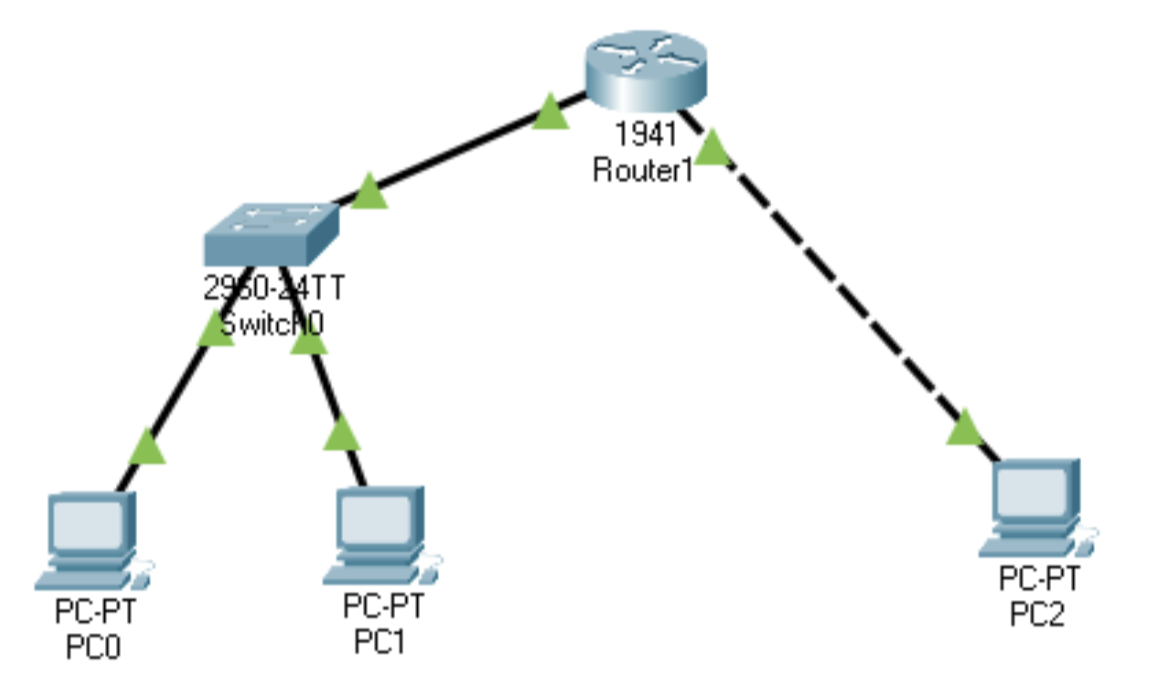
\includegraphics[width=0.9\textwidth]{swrt.png} \\
    {\small \textbf{Figure 9:} Switch to Router Connection in Cisco Packet Tracer}
\end{center}

\subsection{Basic Configuration Steps}
Assume the following:
\begin{itemize}
    \item Switch port: FastEthernet0/1
    \item Router port: GigabitEthernet0/0
    \item Subnet: 192.168.1.0/24
\end{itemize}

\textbf{Step 1: Configure the Router Interface}
\begin{verbatim}
Router> enable
Router# configure terminal
Router(config)# interface gig0/0
Router(config-if)# ip address 192.168.1.1 255.255.255.0
Router(config-if)# no shutdown
\end{verbatim}

\textbf{Step 2: Connect Devices}
\begin{itemize}
    \item Use a straight-through cable from the router's GigabitEthernet0/0 to the switch's FastEthernet0/1.
    \item Ensure devices connected to the switch (like PCs) are in the same subnet, e.g., 192.168.1.X, with default gateway set to 192.168.1.1 (router's IP).
\end{itemize}

\textbf{Step 3: Test the Network}
\begin{itemize}
    \item From any PC connected to the switch, open the command prompt and ping the router’s IP address:
    \begin{verbatim}
    ping 192.168.1.1
    \end{verbatim}
    \item Successful replies confirm the switch-to-router connection is functional.
\end{itemize}

\subsection{Use in Lab Practice}
In our lab, the switch-to-router connection was used to simulate a basic office LAN setup. By connecting the switch to a router and configuring the correct IP addressing, we enabled PCs connected to the switch to access other networks via the router. This helped us understand how routers manage traffic and how switches extend network connectivity within a LAN.

\newpage

\section{OSI Model}
The \textbf{OSI (Open Systems Interconnection) Model} is a conceptual framework developed by the International Organization for Standardization (ISO) that standardizes the functions of a telecommunication or computing system into seven distinct layers. This model helps different networking systems to communicate with each other, regardless of their underlying architecture.

\subsection{Purpose of the OSI Model}
\begin{itemize}
    \item Provides a universal standard for networking hardware and software.
    \item Helps in troubleshooting by isolating network problems layer by layer.
    \item Supports interoperability between various types of systems and technologies.
\end{itemize}

\subsection{The Seven Layers of the OSI Model}

\begin{enumerate}
    \item \textbf{Application Layer (Layer 7)}\\
    This is the topmost layer that interacts directly with user applications. It provides services such as email, file transfer, and web browsing (e.g., HTTP, FTP, SMTP).

    \item \textbf{Presentation Layer (Layer 6)}\\
    Responsible for translating data formats, data encryption/decryption, and compression. It ensures that data is readable by the receiving system (e.g., JPEG, MPEG, SSL/TLS).

    \item \textbf{Session Layer (Layer 5)}\\
    Manages sessions between applications. It establishes, maintains, and terminates connections between devices (e.g., NetBIOS, RPC).

    \item \textbf{Transport Layer (Layer 4)}\\
    Provides reliable data transfer through flow control, error checking, and segmentation (e.g., TCP, UDP).

    \item \textbf{Network Layer (Layer 3)}\\
    Handles data routing, packet forwarding, and logical addressing (IP addressing). Routers operate at this layer (e.g., IP, ICMP).

    \item \textbf{Data Link Layer (Layer 2)}\\
    Manages physical addressing (MAC addresses), error detection, and frame delivery. Switches operate at this layer (e.g., Ethernet, PPP).

    \item \textbf{Physical Layer (Layer 1)}\\
    Deals with the physical connection between devices including cables, switches, voltages, and pin layouts. It transmits raw bit streams over a physical medium.
\end{enumerate}

\begin{center}
    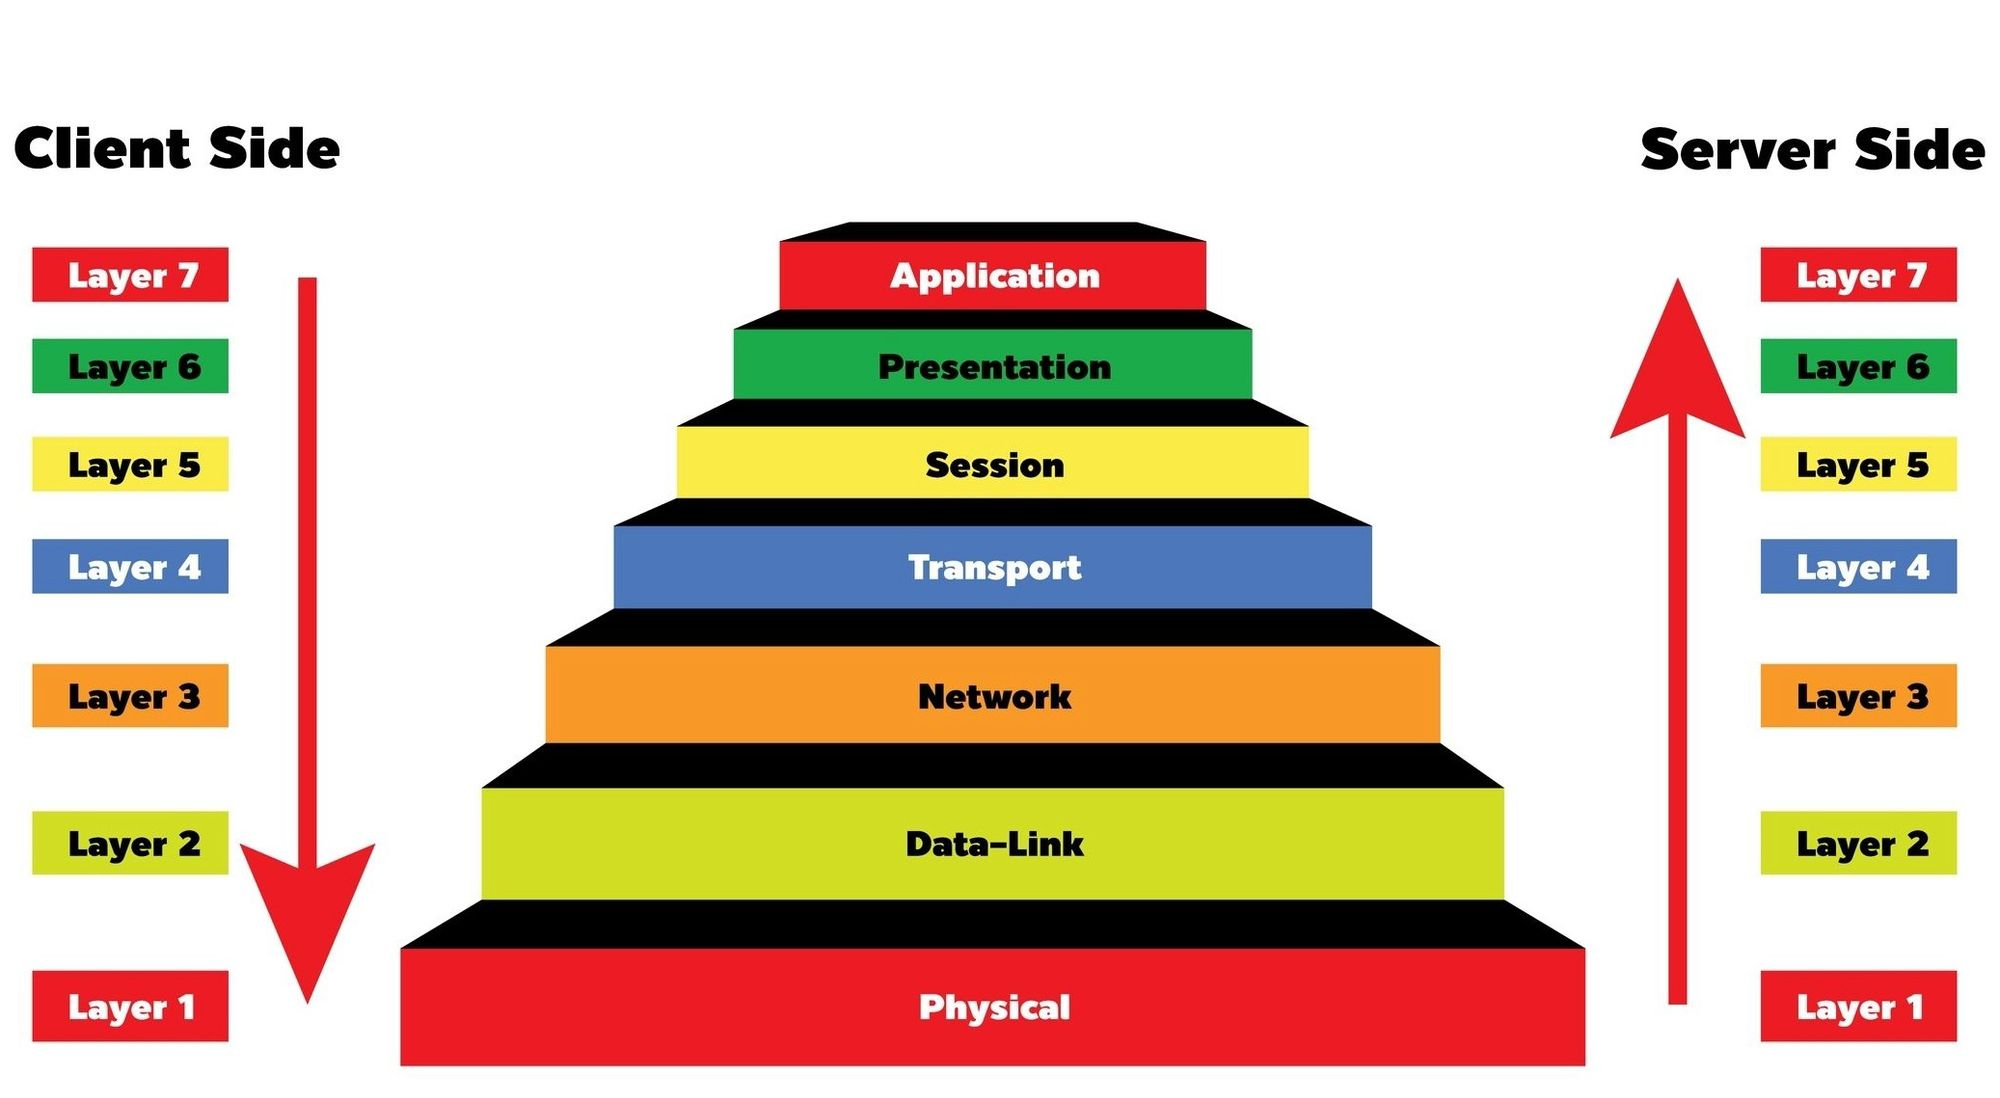
\includegraphics[width=1\textwidth]{OSI.jpg} \\
    {\small \textbf{Figure 10:} OSI Model} \\
\end{center}

\subsection{Mnemonic to Remember the Layers}
\textbf{"All People Seem To Need Data Processing"} (from Layer 7 to Layer 1). \\

\subsection{OSI Model in Networking Labs}
In our networking lab, the OSI Model helped us to understand and troubleshoot communication between devices. For example:
\begin{itemize}
    \item When a PC failed to ping another device, we checked Layer 1 (cable), Layer 2 (MAC), and Layer 3 (IP).
    \item During router configuration, we mainly worked with Layer 3 (Network Layer).
    \item Switch configuration tasks related to Layer 2 (Data Link Layer). \\
\end{itemize}
\newpage
\section{Conclusion}
In conclusion, this lab provided a practical and insightful exploration into the foundational hardware and configurations used in modern computer networks. By working hands-on with tools such as cable tracers, cable testers, and various types of networking cables, we gained essential skills in identifying, connecting, and troubleshooting physical network components. The understanding and application of the T-568B wiring standard were especially important for ensuring correct cable assembly and communication between devices.\\
Moreover, the lab enabled us to explore vital networking equipment, including switches, routers, fiber optic cables, and SFP modules. Through router configurations involving Dynamic NAT and DHCP, we learned how data is dynamically translated and IP addresses are distributed, emphasizing the role of logical configurations in real-time networking. The demonstration of switch-to-router connections further reinforced our grasp of both physical and logical connectivity.\\
The introduction and discussion of the OSI Model allowed us to contextualize each hardware and protocol interaction within a structured framework. This layered approach to understanding network behavior proved invaluable when diagnosing connectivity issues and planning network architecture.\\
Overall, the lab successfully bridged theoretical networking concepts with their real-world applications, enhancing both our knowledge and confidence in setting up, maintaining, and troubleshooting basic to intermediate network infrastructures.\\

\end{document}
